%----------------------------------------------------------------------------
\chapter{Preliminaries}\label{sect:preliminaries}
%----------------------------------------------------------------------------
\label{chap:preliminaries}
The current chapter introduces the basic concepts of \modeldriven engineering (MDE) via a motivating example from the domain of software modeling. It also summarizes the major features and capabilities of the \eiq graph pattern matching framework.

%----------------------------------------------------------------------------
\section{A motivating example: code smell detection in program code}
%----------------------------------------------------------------------------
\label{sec:example}
In order to ensure code quality, and maintainability, several programing rules should be followed when creating a computer program. However, there are several typical mistakes that developers make. These so-called code smells (or in other words anti-patterns) can efficiently be detected by using code queries. For such purposes many advanced techniques use the \emph{abstract syntax graph} (ASG) representation of a program. With the ASG synthesized from the code, graph pattern matching can be the underlying method to execute a query on the software.

Considering this application as a motivating example, we use the \emph{domain of program ASGs}, the \emph{Catch problem} code smell from~\cite{DBLP:journals/infsof/UjhelyiSHCVVF15} to pattern matching related tasks in details throughout this work. Source code of Java programs serve as the subject of this problem, and its definition is the following: in a \texttt{catch} block there is an \texttt{instanceof} check for the type of the \texttt{catch} block parameter. Instead of the \texttt{instanceof} check a new \texttt{catch} block should be added for the checked type and the body of the conditional has to be moved there. 

To demonstrate this code smell, we placed a short Java code fragment in \autoref{lst:javaexample}. In this snippet, a \texttt{try-catch} block surrounds the \texttt{FileInputStream} object creation. In line 2, a checked exception of type \texttt{FileNotFoundException} may be thrown, but the programmer should also prepare for other kinds of (unchecked) exceptions as well, e.g., \texttt{NullPointerException}. In this case, additional \texttt{catch} blocks accepting parameters of different types should be implemented instead of adding only one catch block, and using the \texttt{instanceof} operator on the thrown object.
\begin{figure}[!htp]
	\listingjava{javaexample}{Java code snippet containing code smell}
\end{figure}


%----------------------------------------------------------------------------
\section{Foundations of \modeldriven engineering}
%----------------------------------------------------------------------------
\label{sec:mde}

The aim of \modeldriven engineering is to increase development efficiency by creating various models of the system under development. These models help focusing on the important design decisions, and (ideally) they omit unnecessary details. In terms of software development, several frequently used representations of a program have a graph-like structure, \eg class diagram, component diagram, state machine, and the ASG, as in our running example. The models can be then used for different purposes including source code generation, test case derivation, and even simulation.

A huge advantage of graph-like representation is that there are many analysis techniques, which can be applied to detect errors in models~\cite{DBLP:conf/kbse/CsertanHMPPV02, bur}. Additionally, the definition of graph patterns can be done in a very concise, and expressive way. 


\subsection{Metamodeling}

As it is described in~\cite{osemerath/msc}, metamodels define available concepts, that can be used to build up the instance model containing only elements typed by the metamodel. These concepts can also have attributes in order to enrich the expressiveness of the language. In a metamodel, relations define connections between concepts, and links are the instances of such a relation. Via the allowed relations, the metamodel also defines the structure of the models.


\subsection{Eclipse Modeling Framework}
\label{sec:EMF}

%TODO shorten description?

This section about Eclipse Modeling Framework (EMF) is based on~\cite{ahorvath/msc}. EMF is a Java framework and code generation facility for building tools and other applications based on a structured model. EMF provides a metamodel (called ECore) for describing structured models. Using these structured models EMF provides a toolkit and runtime support to produce a set of Java classes representing the model in the Java Virtual Machine (JVM), a set of adapter classes that enable viewing, and a basic editor. As EMF already supports a large set of modeling constructs, our discussion mainly focuses on the ECore meta- and instance models and follows~\cite{Budinsky2003}.

%ECore, which is essentially the class diagram subset of UML, is based on the Object Management Group’s (OMG) Meta Object Facility (MOF) specification. 

A simplified ECore model is depicted in \autoref{fig:ecore} in order to demonstrate the most important elements of the metamodel.

\begin{itemize}
	\item \texttt{EClass} models classes themselves. Classes are identified by their name and can	contain a number of attributes and references. To support inheritance, a class can refer to a number of other classes as its supertypes.
	
	\item \texttt{EAttribute} models attributes, the components of an object’s data. They are identified by their name, and they have a type.
	
	\item \texttt{EDataType} models the types of attributes, representing object data types that are defined in Java, but not in EMF. Data types are also identified by their name.

	\item \texttt{EReference} is used in modeling associations between classes; it models one end of such an association. Like attributes, references are identified by their name and have a type.
\end{itemize}

\begin{figure}[!htp]
	\centering
	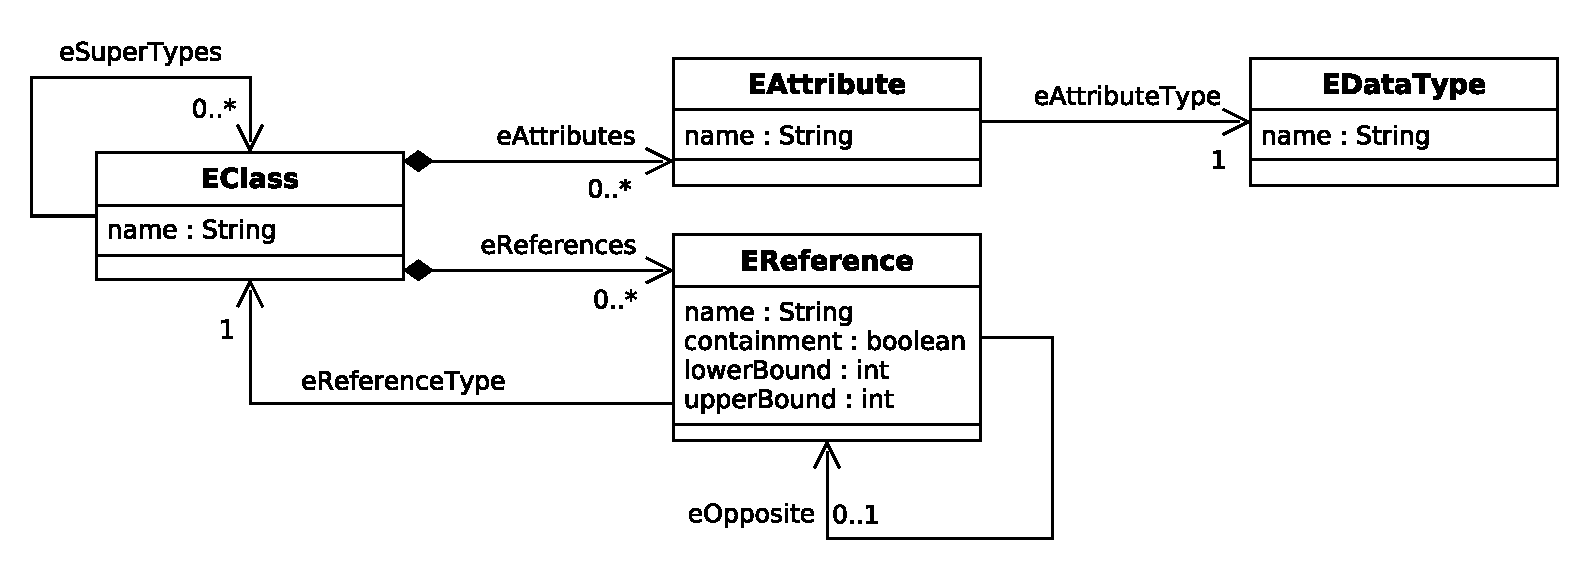
\includegraphics[width=\textwidth]{figures/pdfs/ecore-kernel.pdf}
	\caption{The ECore metamodel}
	\label{fig:ecore}
\end{figure}


\subsubsection{Extension of the ECore}
From an ECore model, the generator of EMF can create a corresponding set of Java implementation classes. Every generated EMF class extends from the framework base class, \eobject, which enables the objects to be integrated and appear in the EMF runtime environment. \eobject provides an efficient reflective API for accessing the properties of the object generically. In addition, change notification is an essential property of every \eobject and an adapter framework can be used to support extension to the objects.

The reflective API~\cite{EMFAPI} \label{sec:emf-reflection}in EMF enables to manipulate all attributes and references attached to the \eobject by using the \texttt{eSet} and \texttt{eGet} functions. This is conceptually equivalent to \texttt{java.lang.reflect.Method.invoke()} Java method, though it is much more efficient in the aspect of performance.
	
 Notification observers (or listeners) in EMF are called adapters~\cite{EMFAdapter} because in addition to their observer status, they are often used to extend the behavior (that is, support additional interfaces without subclassing) of the object they are attached to. An Adapter, as a simple observer, can be attached to any \eobject by simply adding the adapter to the \texttt{eAdapters} list of the \eobject. This Adapter implements a function called \texttt{notifyChanged}, which is called any time when the \eobject, which contains the Adapter, is manipulated. All information about the manipulation is held by a notification object which is the input parameter of the \texttt{notifyChanged} function. This adapter is responsible for sending the notifications to the \texttt{EMFInstanceAdapter} manager class.



\subsubsection{Example EMF metamodel and model of a program ASG}

As an running example, the an EMF metamodel is shown in \autoref{fig:example-mm}, as exported from \emph{ECoreTools}~\cite{ecoretools}. The main parts of the metamodel are the following:

\begin{itemize}
	\item \texttt{Expression} is the superclass for every expression type,
	
	\newcommand{\javaCode}[1]{\lstinline[language=java,keepspaces=true,basicstyle=\ttfamily]!#1!}
	
	
	\item instances of \texttt{Unary} represent expressions that only accept up to one expression as their operand,
	\item instances of \texttt{InstanceOf} stand for \texttt{instanceof} operators in the code,
	\item instances of \texttt{Identifier} represent valid Java identifiers in the ASG,
	\item \texttt{Named} is a superclass of any valid Java ASG element, that is supplied with a name (except for \texttt{Identifier} to avoid loops via the \texttt{refersTo} relation),
	\item instances of \texttt{Parameter} represent parameters in the program, and
	\item \texttt{Handler} marks an exception handler \texttt{catch} block for a \texttt{try-catch} construction in the ASG.
\end{itemize}

\begin{figure}[!htp]
	\centering
	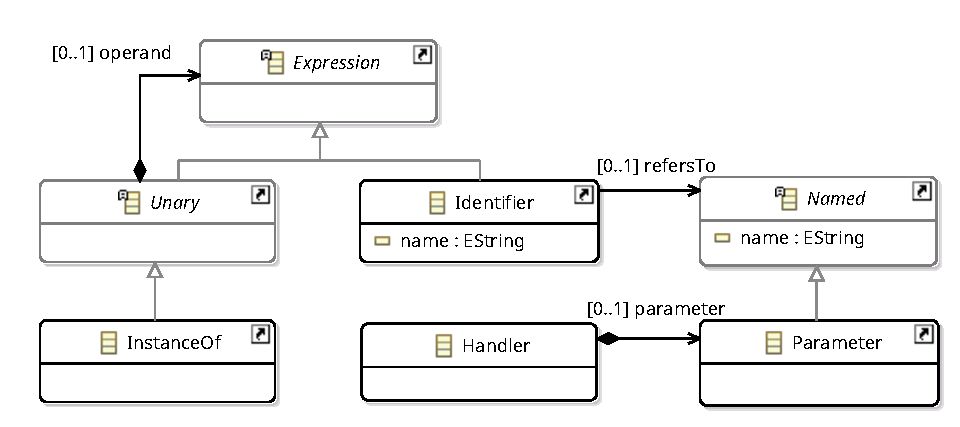
\includegraphics[width=0.9\textwidth]{figures/pdfs/example-metamodel.pdf}
	\caption{EMF metamodel fragment for ASGs}
	\label{fig:example-mm}
\end{figure}

From the explanatory code snippet in \autoref{lst:javaexample}, using the same tool that was used to generate the ASGs of the programs included in~\cite{DBLP:journals/infsof/UjhelyiSHCVVF15}, we obtained the EMF model.
%presented in \autoref{fig:example-instancemodel}, opened in the generated EMF model editor in Eclipse. 
We include a hand drawn version of the instance model in \autoref{fig:example-instancemodel-handdrawn}. It uses simplified object names and applies some trivial abbreviations of the type names. 
%Under every the name and type of every object we included the corresponding line numbers from \autoref{lst:javaexample}. 
Each node in \autoref{fig:example-instancemodel-handdrawn} is adorned with its corresponding line number from  \autoref{lst:javaexample}.
We also used four different colors for the \texttt{Expression}, \texttt{Named}, \texttt{Statement} and \texttt{Handler} types. The subtypes of these types are marked with the same color as the corresponding supertype. Some element types are not shown above in the metamodel fragment, for they would only complicate the structure, and would not help the comprehension of the example. However, we include a more detailed, but still incomplete metamodel in \autoref{fig:example-extended-mm} in the Appendix.

%\begin{figure}[!htp]
%	\centering
%	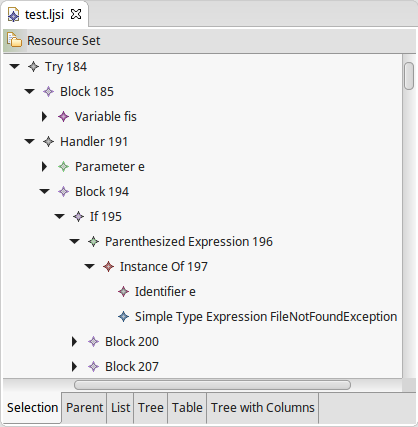
\includegraphics[scale=0.5]{figures/instancemodel-emfeditor}
%	\caption{The EMF instance model opened in the generated editor}
%	\label{fig:example-instancemodel}
%\end{figure}


\begin{figure}[!htp]
	\centering
	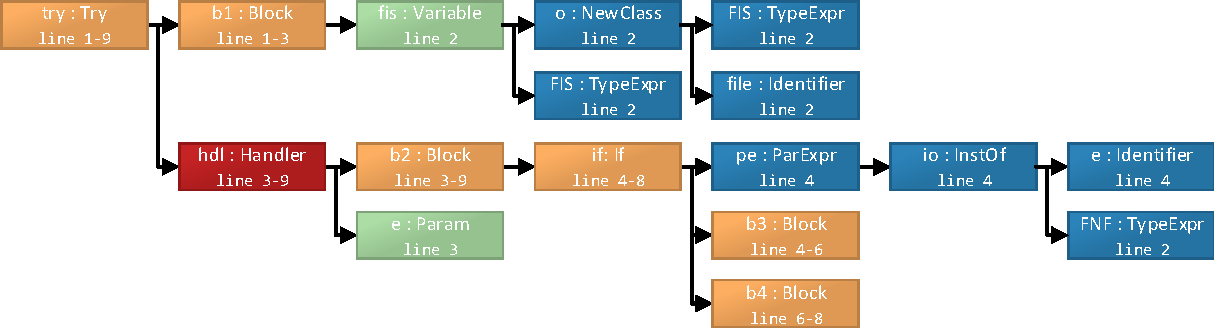
\includegraphics[width=\textwidth]{figures/pdfs/instance_model.pdf}
	\caption{The ASG representation of the example code snippet}
	\label{fig:example-instancemodel-handdrawn}
\end{figure}


%----------------------------------------------------------------------------
\section{Implementing model queries using graph patterns}
%----------------------------------------------------------------------------
\label{sec:graphpatterns}


As described in~\cite{DBLP:journals/scp/UjhelyiBHHIRSV15}, graph patterns are graph-like structures that encapsulate a set of constraints regarding the nodes, the attributes of the nodes, and edges. Model queries can be carried out by matching a graph pattern against instance model graphs. During the matching process the objective is to find suitable model elements that satisfy all constraints of the graph pattern. According to~\cite{DBLP:conf/icmt/BergmannURV11}, \eiq is a framework with a \emph{language for defining declarative queries over EMF models}, and a \emph{runtime engine for executing them efficiently without manual coding}. 

%TODO from what to what and how


\subsection{\eiq pattern language}
\label{sec:patternlanguage}
The framework has its own highly declarative pattern language called IncQuery Pattern Language (IQPL). The language is similar to Datalog, which is a subset of Prolog. As stated in~\cite{DBLP:conf/icmt/BergmannURV11}, the graph pattern based query language of \eiq references \texttt{EClasses} as node types, \texttt{EReferences} and \texttt{EAttributes} as edge types. Pattern variables will be mapped to \texttt{EObjects} of the instance model or attribute values. It is important to add that the language does not specify the order of constraint evaluation.

%\todo{introduce (advanced) language constructs: transitive closure, neg find, count find, check expression, eval}


Based on~\cite{sosym-dslvalidation}, we provide a short summary of the constraints supported by the IQPL:

\begin{itemize}
	\item \textbf{Classifier constraint:} checks if a variable is an instance of an \texttt{EClass}.
	\item \textbf{Path constraint:} requires a specific reference, an attribute, or a path of reference and attribute sequence between two variables.
	\item \textbf{Equality constraint:} specifies that two variables have to be mapped to the same model element.
	\item \textbf{Pattern call constraint:} enables the composition of multiple patterns. The \emph{positive pattern call} refers to another pattern and specifies that the called pattern must be satisfied in the context of the actual parameters. Additionally, a pattern may define a \emph{negative application condition} (\texttt{neg} keyword), which means that the target pattern is disallowed to have a valid match along the actual parameters. Using the \texttt{count} keyword, \eiq can save the \emph{number of matches} to a variable. 
	\item \textbf{Binary transitive closure}: it is possible to describe the \emph{transitive closure} of a two-parameter pattern by the \texttt{+} symbol.
	\item \textbf{Check constraint:} evaluates a specific attribute expression on the variables of the pattern and accept matches only if the result of attribute condition is true.
	\item \textbf{Eval constraint:} evaluates an expression defined inside the constraint. The return value of the evaluation will be stored in a variable.
\end{itemize}



In order to demonstrate the basic capabilities and structural constraints of the language, \autoref{lst:catch} shows the example catch finder problem formulated in IQPL. It introduces two patterns, \catchproblem and \handlervar, both with two symbolic parameters. There are type constraints applied to the parameters: the substitutions of \texttt{cBlock} need to be of type \texttt{Handler}, while \texttt{insOf} is expected to be an \texttt{InstanceOf}. 

% This prevents the listing to be split between pages
\begin{figure}[!htbp]
	\listingiqpl{catch}{Patterns to detect missing catch clauses} 
\end{figure}

The \catchproblem pattern specifies its match set as a set that holds tuples of type $ \langle \texttt{Handler, InstanceOf} \rangle $ in line 1 using classifier constraints for parameters.  In line 2 the pattern declares that the \texttt{varRef} variable should be subtituted with an instance of \texttt{Identifier}, which is also expressed using a classifier constraint. Line 3 prescribes by a path constraint that the \eobject substituted to \texttt{insOf} should have \texttt{varRef} as its \texttt{operand}. In addition, the pattern also uses a pattern call constraint to reference the \handlervar pattern, and the call will use the substitutions of \texttt{cBlock}, and \texttt{varRef} variables.

The latter pattern will have tuples of $ \langle \texttt{Handler, Identifier} \rangle $ in its match set, according to line 7. Line 8 states that the variable \texttt{cBlock} shall have \texttt{param} as its \texttt{parameter}. In line 9 it is specified that the \eobject substituted into \texttt{param} should be navigable from \texttt{variable} via an instance of the \texttt{refersTo} \texttt{EReference}.




\subsection{Incremental pattern matching}

The \eiq framework initially was designed to provide pattern matching capability for its users, based on an incremental pattern matching algorithm (Rete~\cite{bergmann:thesis-queries}). This approach relies on the idea that along with the computation of the initial match set of each pattern, a data structure is built in the memory. This data structure is then maintained in a way that every change in the underlying model is propagated efficiently, so that the set of matches is updated. In case of EMF models this update mechanism implemented using the efficient EMF notification observers of the framework.

%A generic Rete network structure is depicted in \autoref{fig:rete}. This is essentially a dataflow network, where the input data is located in \emph{input nodes}. Each input node contains 
%
%\begin{figure}[!htp]
%	\centering
%	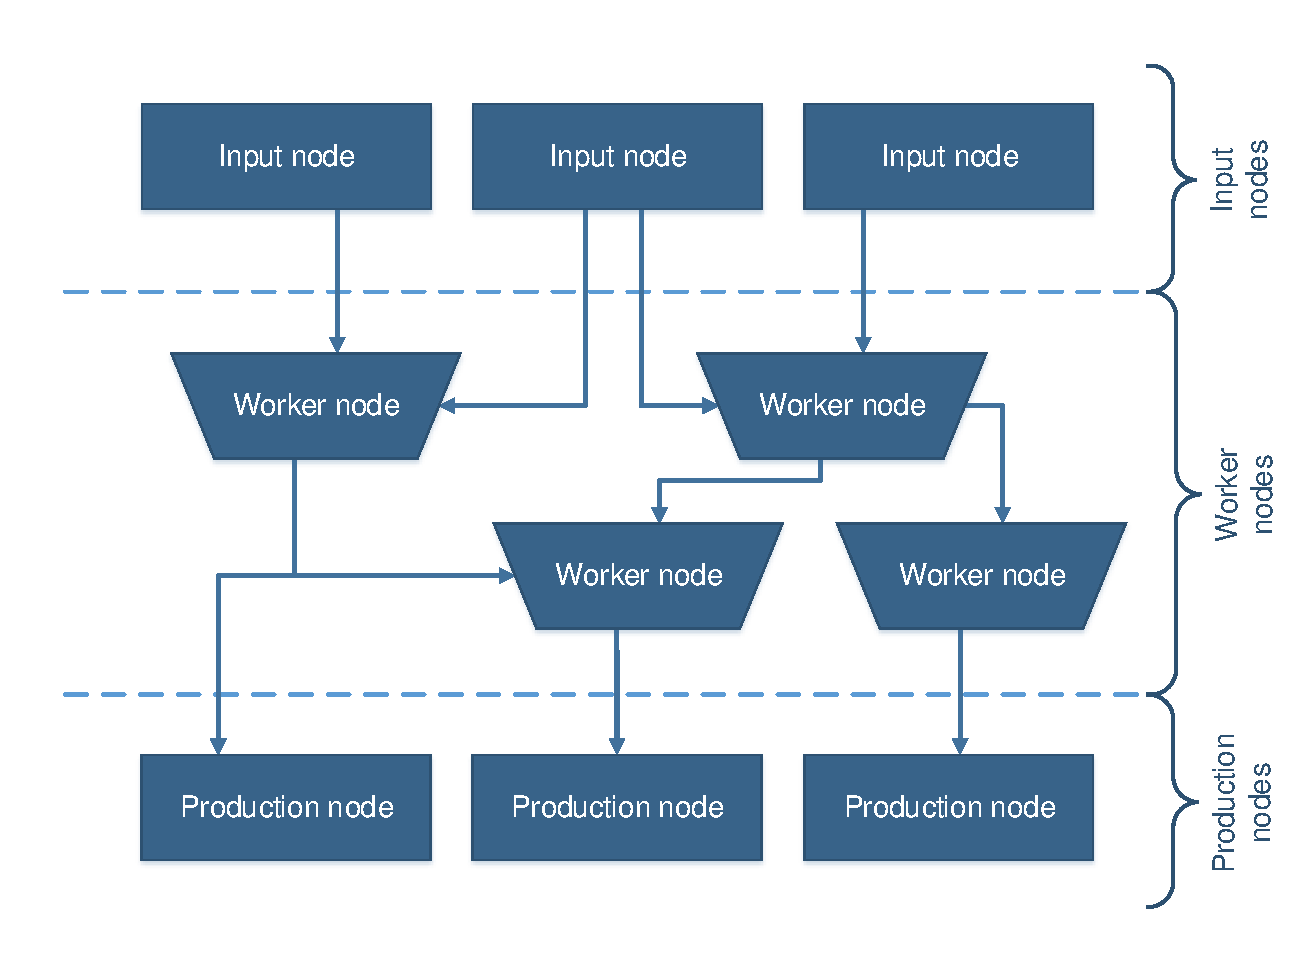
\includegraphics[width=\textwidth]{figures/pdfs/rete.pdf}
%	\caption{Schema for Rete network}
%	\label{fig:rete}
%\end{figure}

To demonstrate this in operation using our example, \autoref{fig:example-rete} depicts a possible  Rete network for the \catchproblem pattern. The Rete network is essentially a dataflow network, where every node contains tuples of arbitrary length. At the top of the diagram rectangles symbolize \emph{input nodes}, which provide input for the network. The second node in the top-left corner is, in addition, a \emph{production node} that means it already holds the match set of the \handlervar pattern. 

\begin{figure}[!htp]
	\centering
	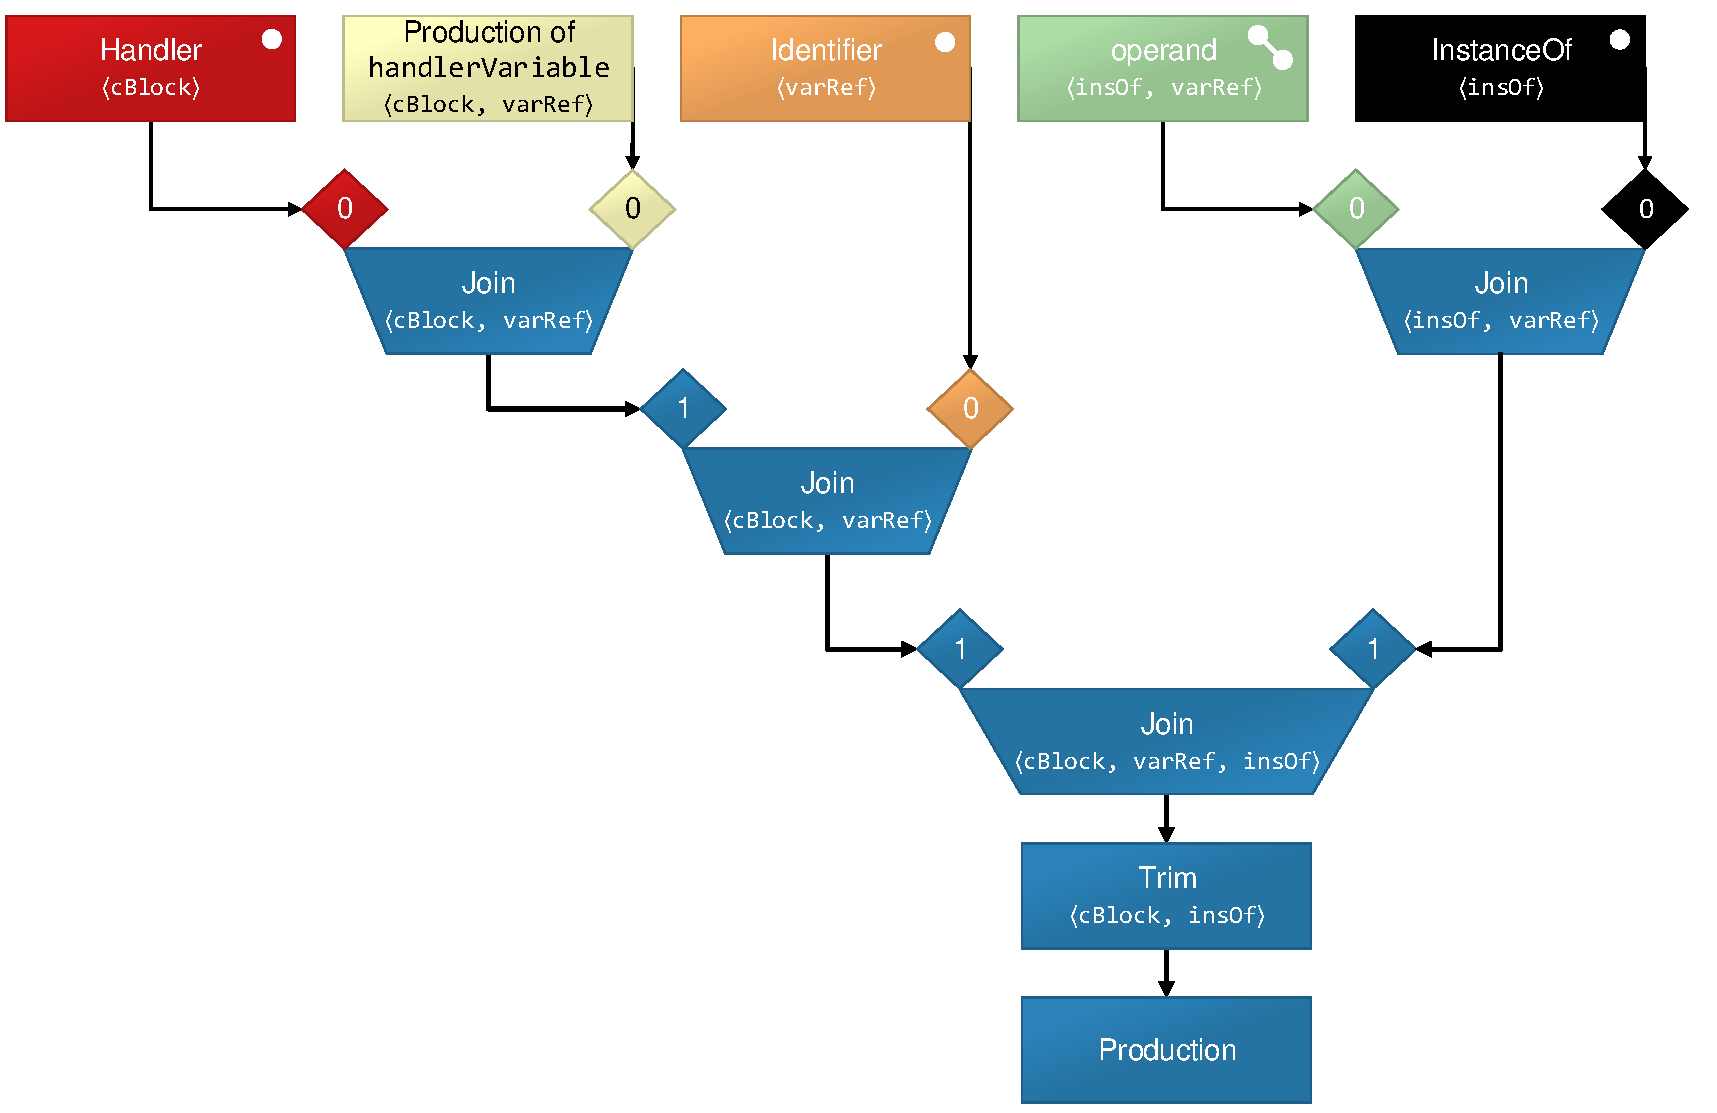
\includegraphics[width=\textwidth]{figures/pdfs/rete-catchProblemFinder-layout.pdf}
	\caption{Rete network for the \catchproblem pattern}
	\label{fig:example-rete}
\end{figure}


Nodes with \emph{Join} annotation are a type of \emph{worker nodes}. They carry out join operation on the input. The diamonds over the worker nodes indicate the operand indices from the previous node. The \emph{Trim} node omits some values from the preceding worker node. In the example, $\langle \texttt{cBlock, varRef, insOf} \rangle $ is trimmed to $\langle \texttt{cBlock, insOf} \rangle $. Finally, \emph{Production} will hold the match set for a pattern.


The main advantage of this solution is the ability to retrieve the match results in constant time after the first evaluation, if the model is unchanged. In case the model changes, the match result update time is proportional to the size of the change, and not the size of the complete model.

In the example, when a new object of type \texttt{Identifier} appears, the change is propagated in the Rete net on a directed path down to the production node. This way matches after small changes in the model are instantly updated.

However, a main drawback of this approach is the memory footprint of the internal data structure. Its size depends on the size of the model and the complexity of the pattern. In certain application scenarios, in which the models themselves are extremely large, this footprint means a bottleneck concerning the usability of the algorithm.


%This summary of the Rete incremental pattern matcher algorithm is based on~\cite{szarnyasg/msc}. The initial version of the algorithm was described in~\cite{DBLP:conf/isca/GuptaFNW86}, and was created for rule-based expert systems. It was adapted and optimized for the Eclipse Modeling Framework by Gábor Bergmann~\cite{bergmanng/msc}. 

%The basis of its operation is an asynchronous network of communicating nodes, which is fundamentally a dataflow network. A generic version of such a structure is depicted in \autoref{fig:rete}. When the algorithm starts, it builds up this network and computes the match set of every pattern. Then, by using notifications from the 

%\begin{figure}[!htp]
%	\centering
%	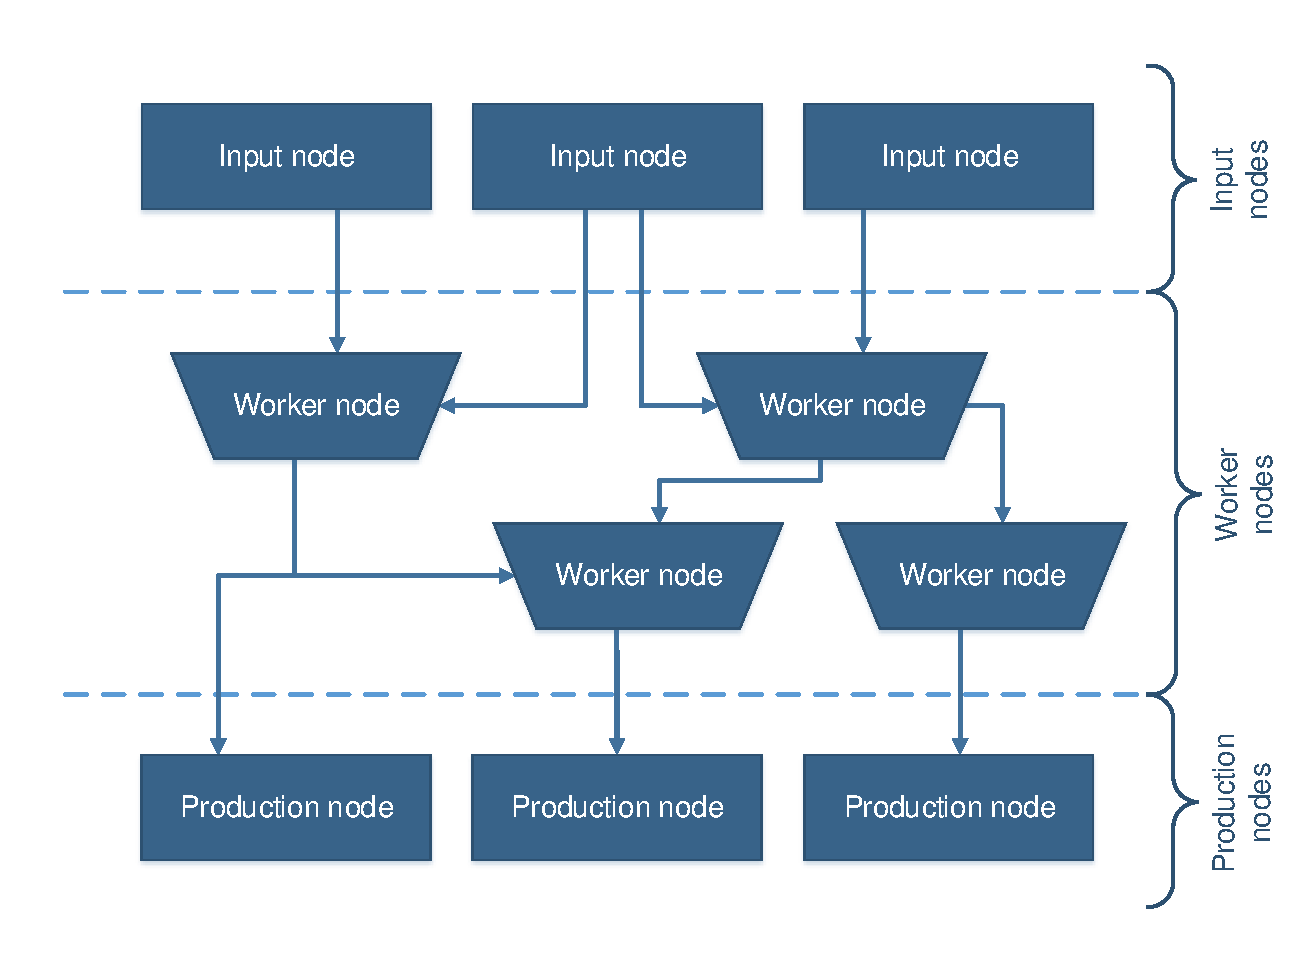
\includegraphics[width=\textwidth]{figures/pdfs/rete.pdf}
%	\caption{The generic stucture of a Rete network}
%	\label{fig:rete}
%\end{figure}
%
%\begin{figure}[!htp]
%	\centering
%	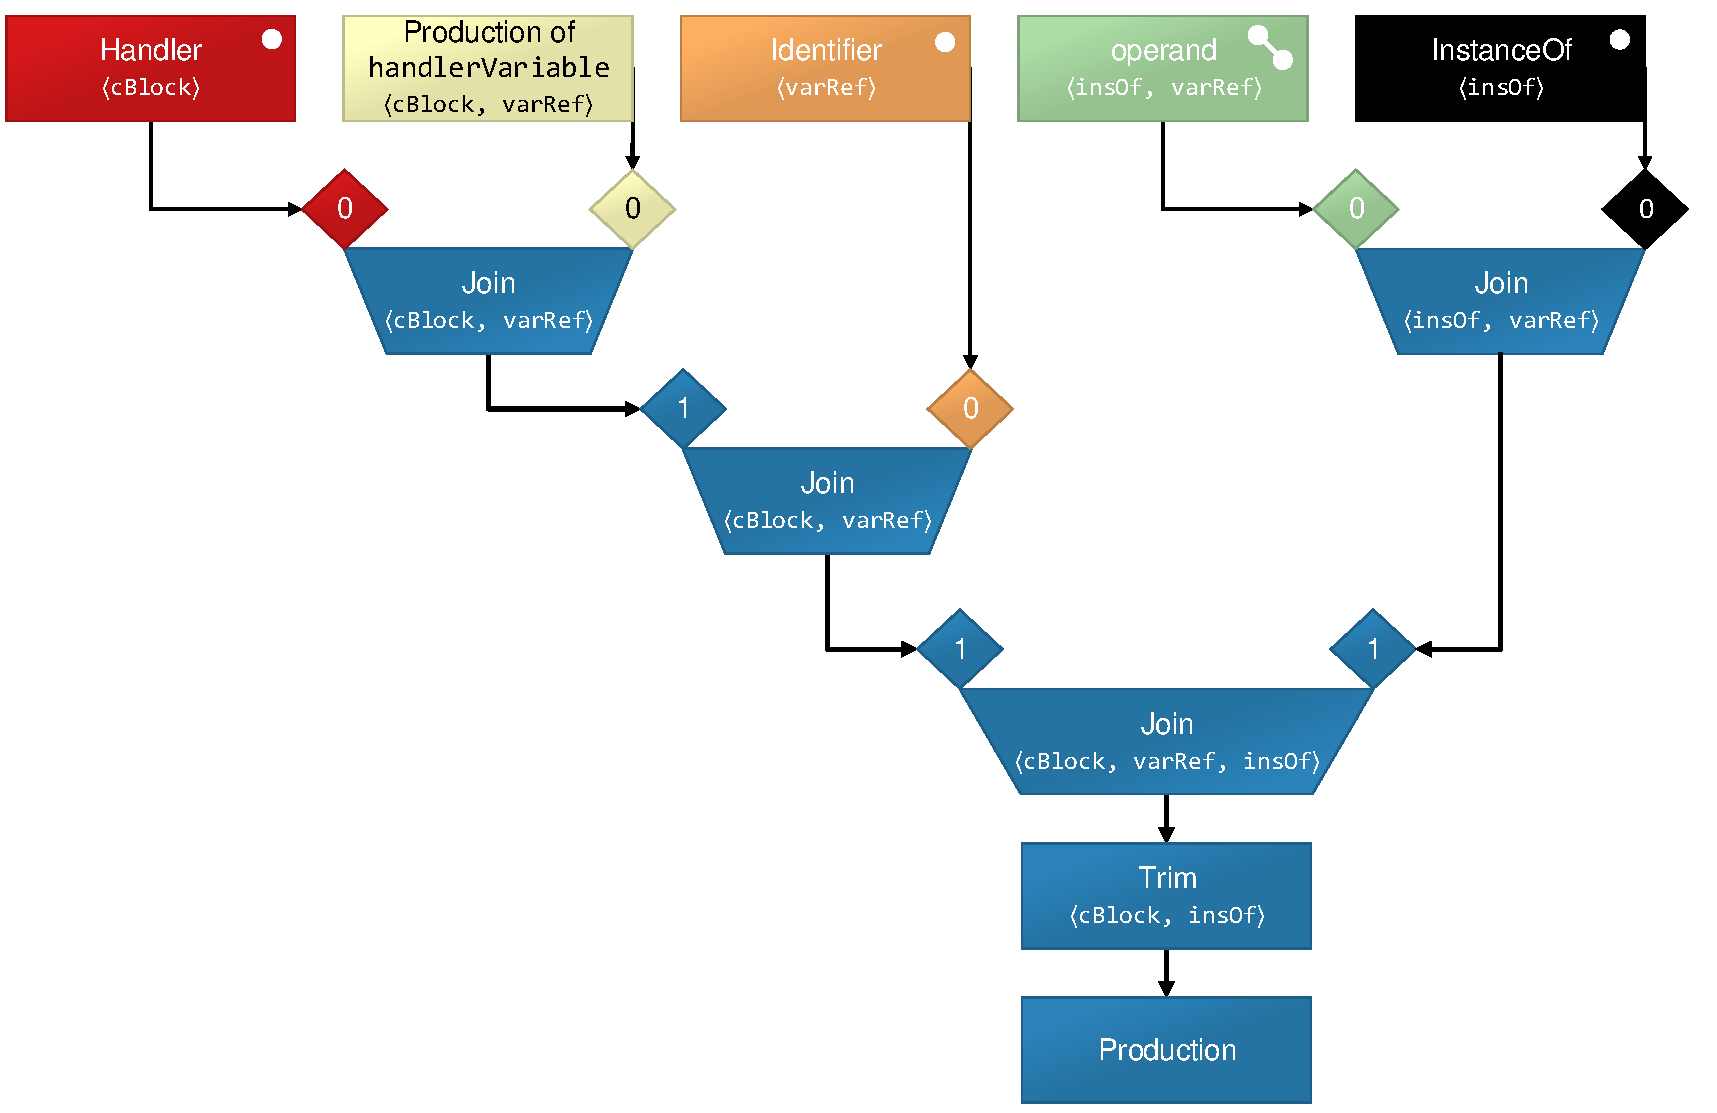
\includegraphics[width=\textwidth]{figures/pdfs/rete-catchProblemFinder-layout.pdf}
%	\caption{The rete network for the catch problem finder query}
%	\label{fig:example-rete}
%\end{figure}
